%%%%%%%%%%%%%%%%%%%%%%
\begin{frame}{Case 1}

\begin{columns}
 \begin{column}{.70\textwidth}
	\begin{center}
		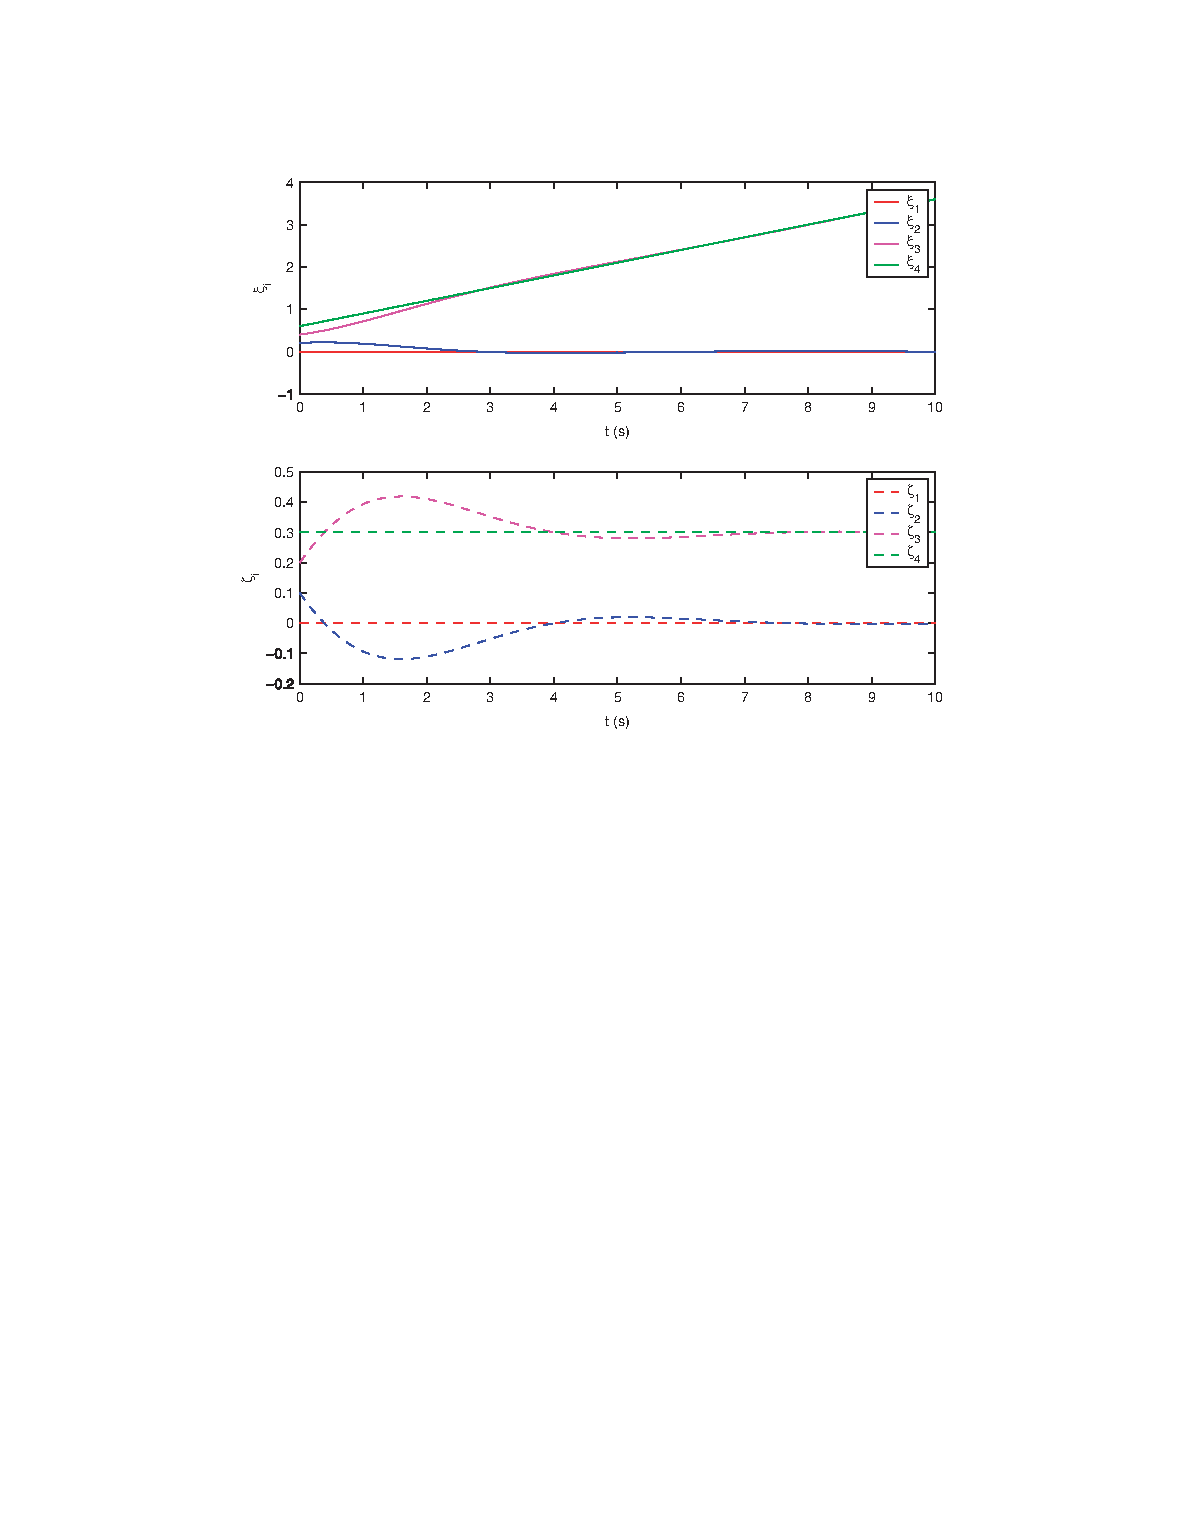
\includegraphics[height=6cm]{images/StatesCase1.pdf}
	\end{center}
	\vskip 0.3cm
 \end{column}

 \begin{column}{.30\textwidth}
	\begin{center}
		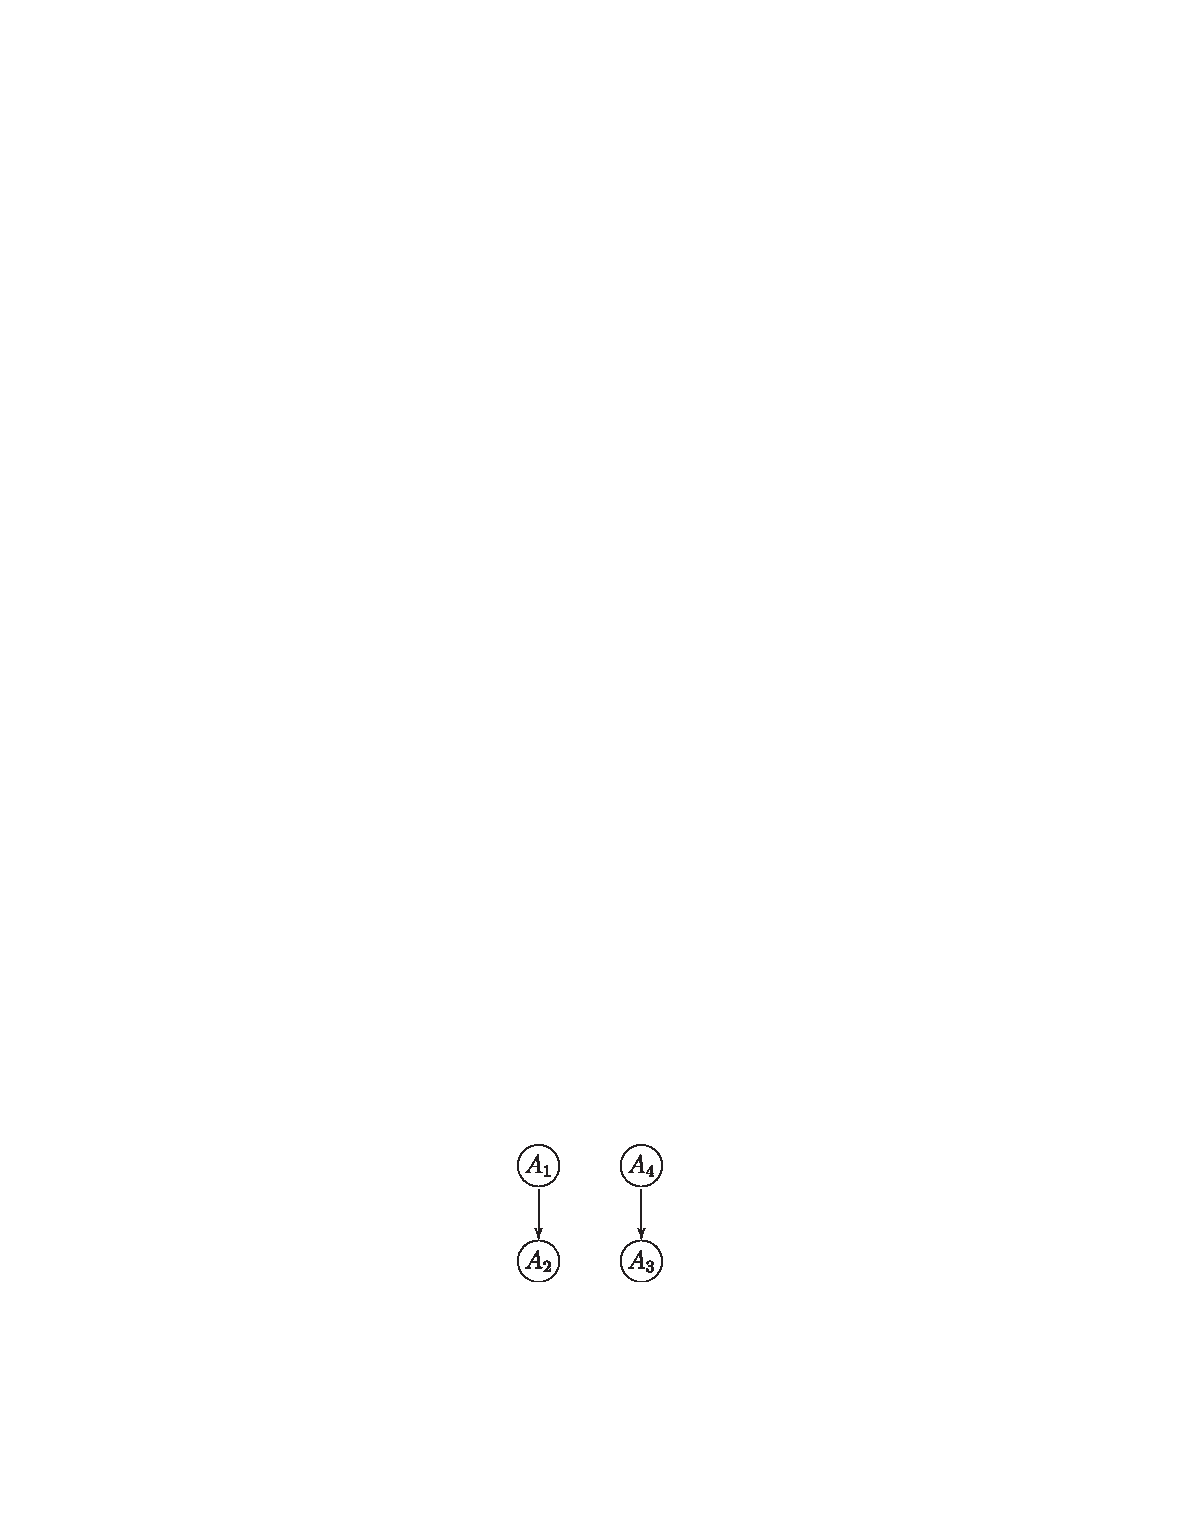
\includegraphics[height=2cm]{images/GraphCase1.pdf}
	\end{center}
	{\textcolor{green!40!black}{\fontsize{13}{15}\textbf{Consensus cannot be achieved}}} 
	since the information states from different groups do not affect one another. 
 \end{column}
\end{columns}
We also know that  L has at least two zero eigenvalues in this case, which in turn implies that $\Gamma$ has at least 
{\textcolor{green!40!black}{\fontsize{13}{15}\textbf{four zero eigenvalues}}}.
\vskip 0.3cm

\end{frame}

%%%%%%%%%%%%%%%%%%%%%%
\begin{frame}{Case 2}

\begin{columns}
 \begin{column}{.70\textwidth}
	\begin{center}
		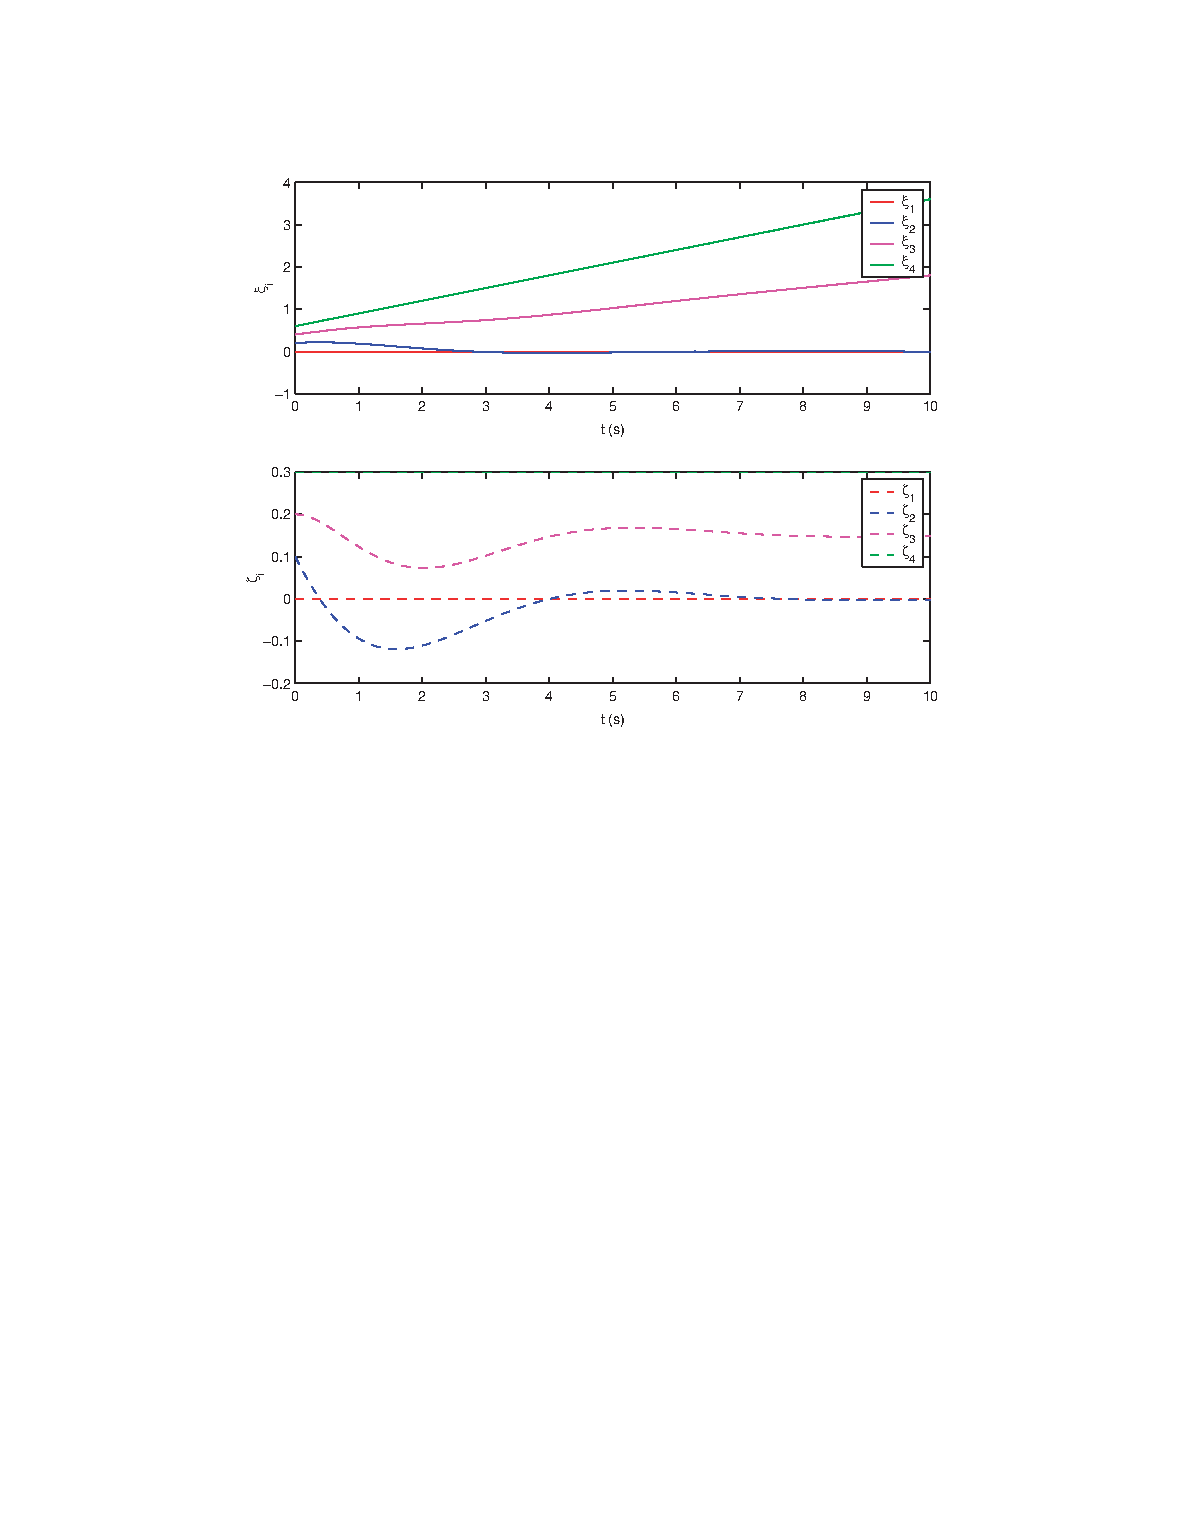
\includegraphics[height=6cm]{images/StatesCase2.pdf}
	\end{center}
	\vskip 0.3cm
 \end{column}
 \begin{column}{.30\textwidth}
 	\vskip 0.3cm
	\begin{center}
		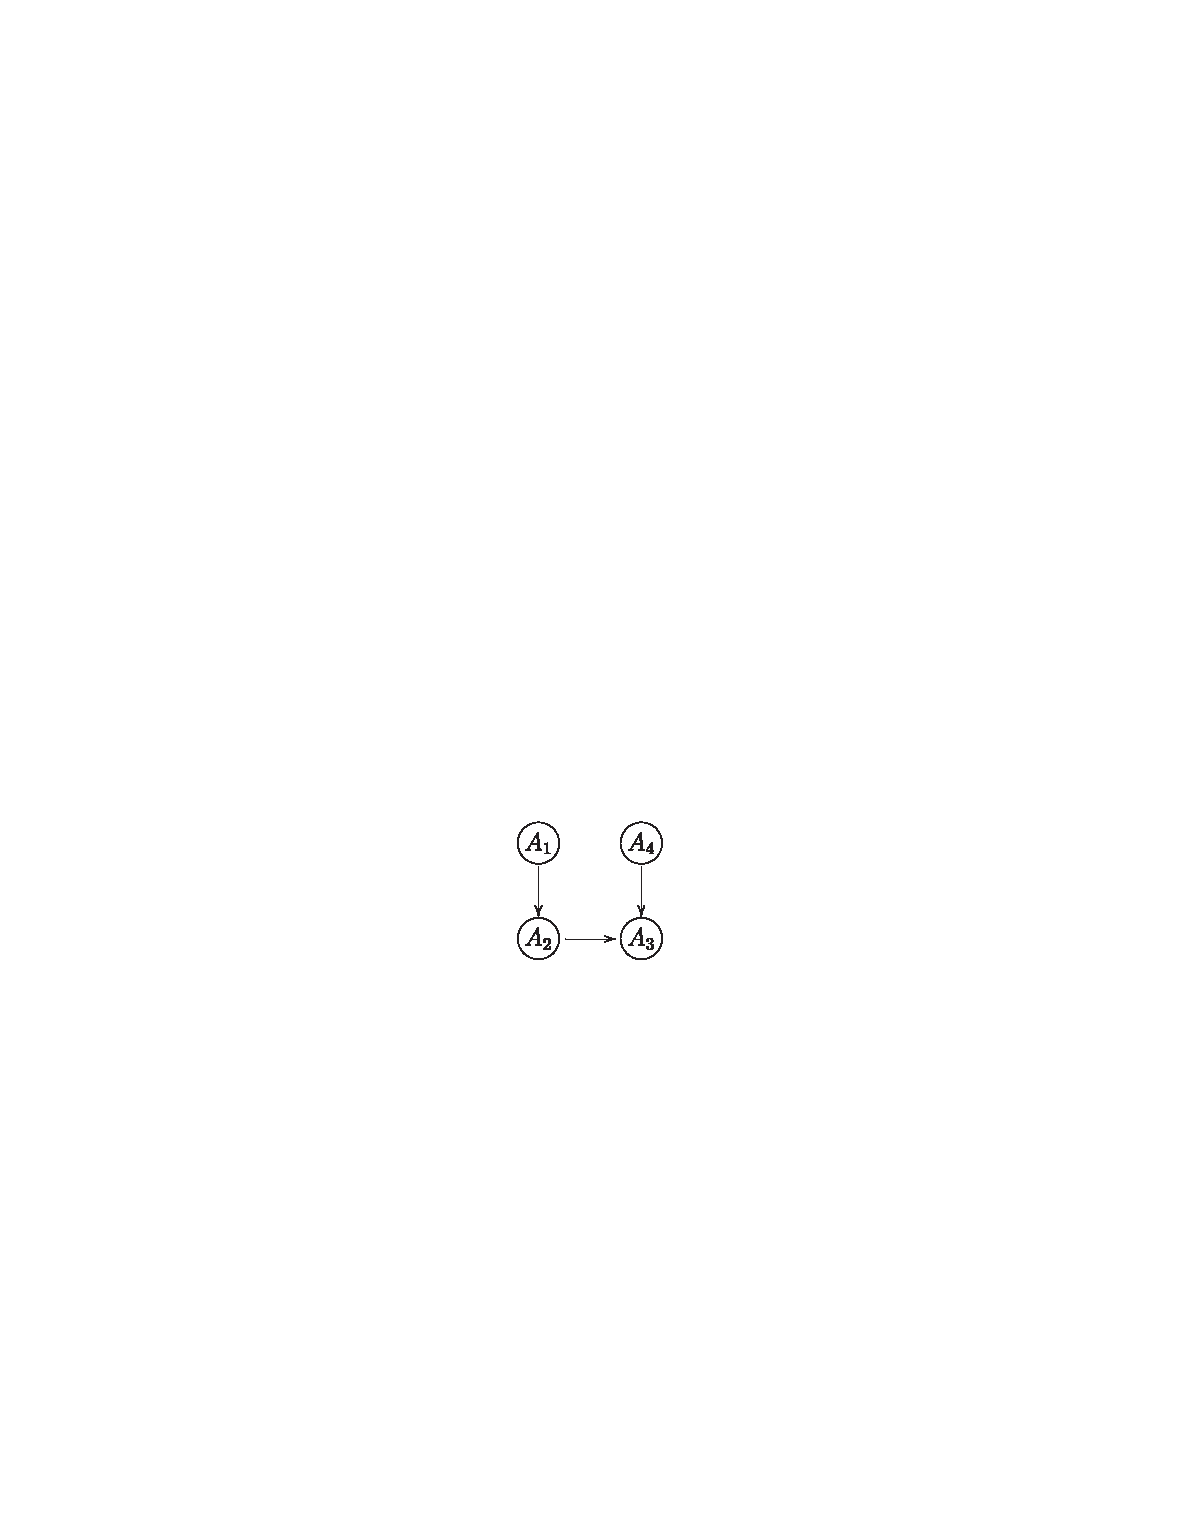
\includegraphics[height=2cm]{images/GraphCase2.pdf}
	\end{center}
	If a vehicle only has outgoing links without incoming ones, we call it a leader.
	Here we have {\textcolor{green!40!black}{\fontsize{13}{15}\textbf{multiple leaders}}}.
 \end{column}
\end{columns}
{\textcolor{green!40!black}{\fontsize{13}{15}\textbf{Consensus cannot be achieved}}} ,  
L has at least two rows with all zero entries in this case, we know that  L has at least two zero eigenvalues, 
which in turn implies that $\Gamma$ 
has at least {\textcolor{green!40!black}{\fontsize{13}{15}\textbf{four zero eigenvalues}}}.
\vskip 0.3cm

\end{frame}

%%%%%%%%%%%%%%%%%%%%%%
\begin{frame}{Case 3}

\begin{columns}
 \begin{column}{.70\textwidth}
	\begin{center}
		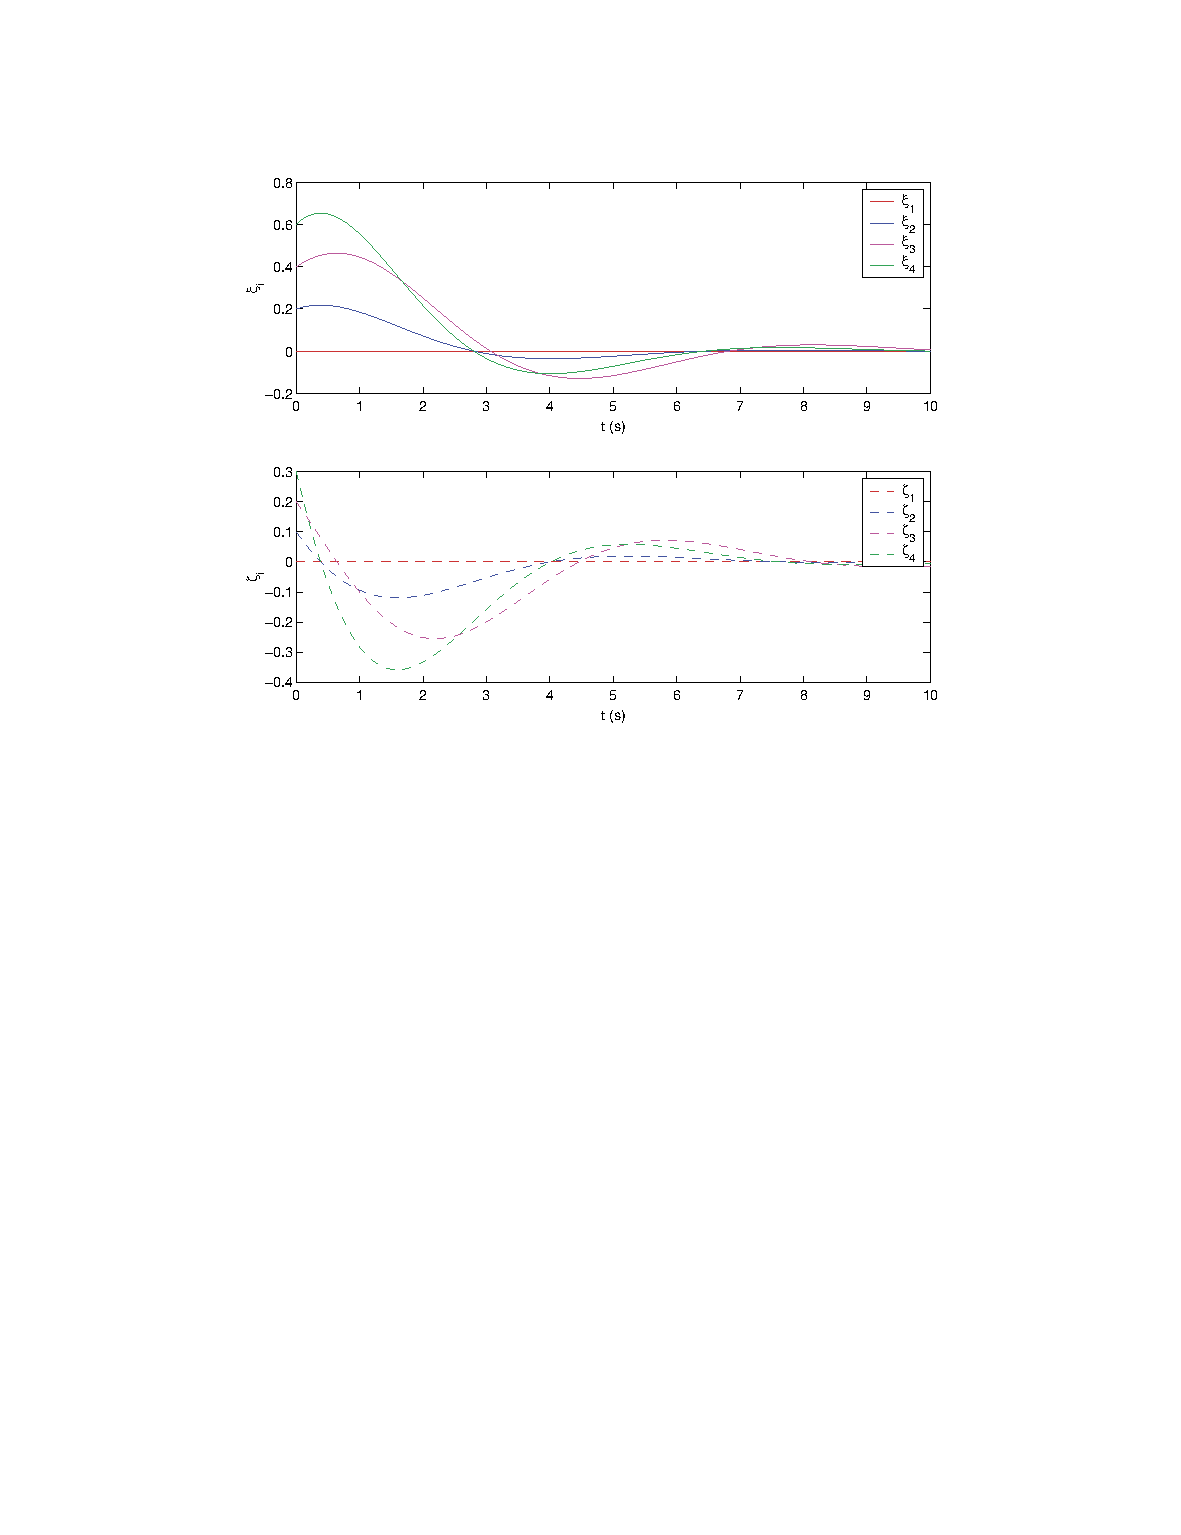
\includegraphics[height=6cm]{images/StatesCase3.pdf}
	\end{center}
	\vskip 0.3cm
 \end{column}
 \begin{column}{.30\textwidth}
 	\vskip 0.3cm
	\begin{center}
		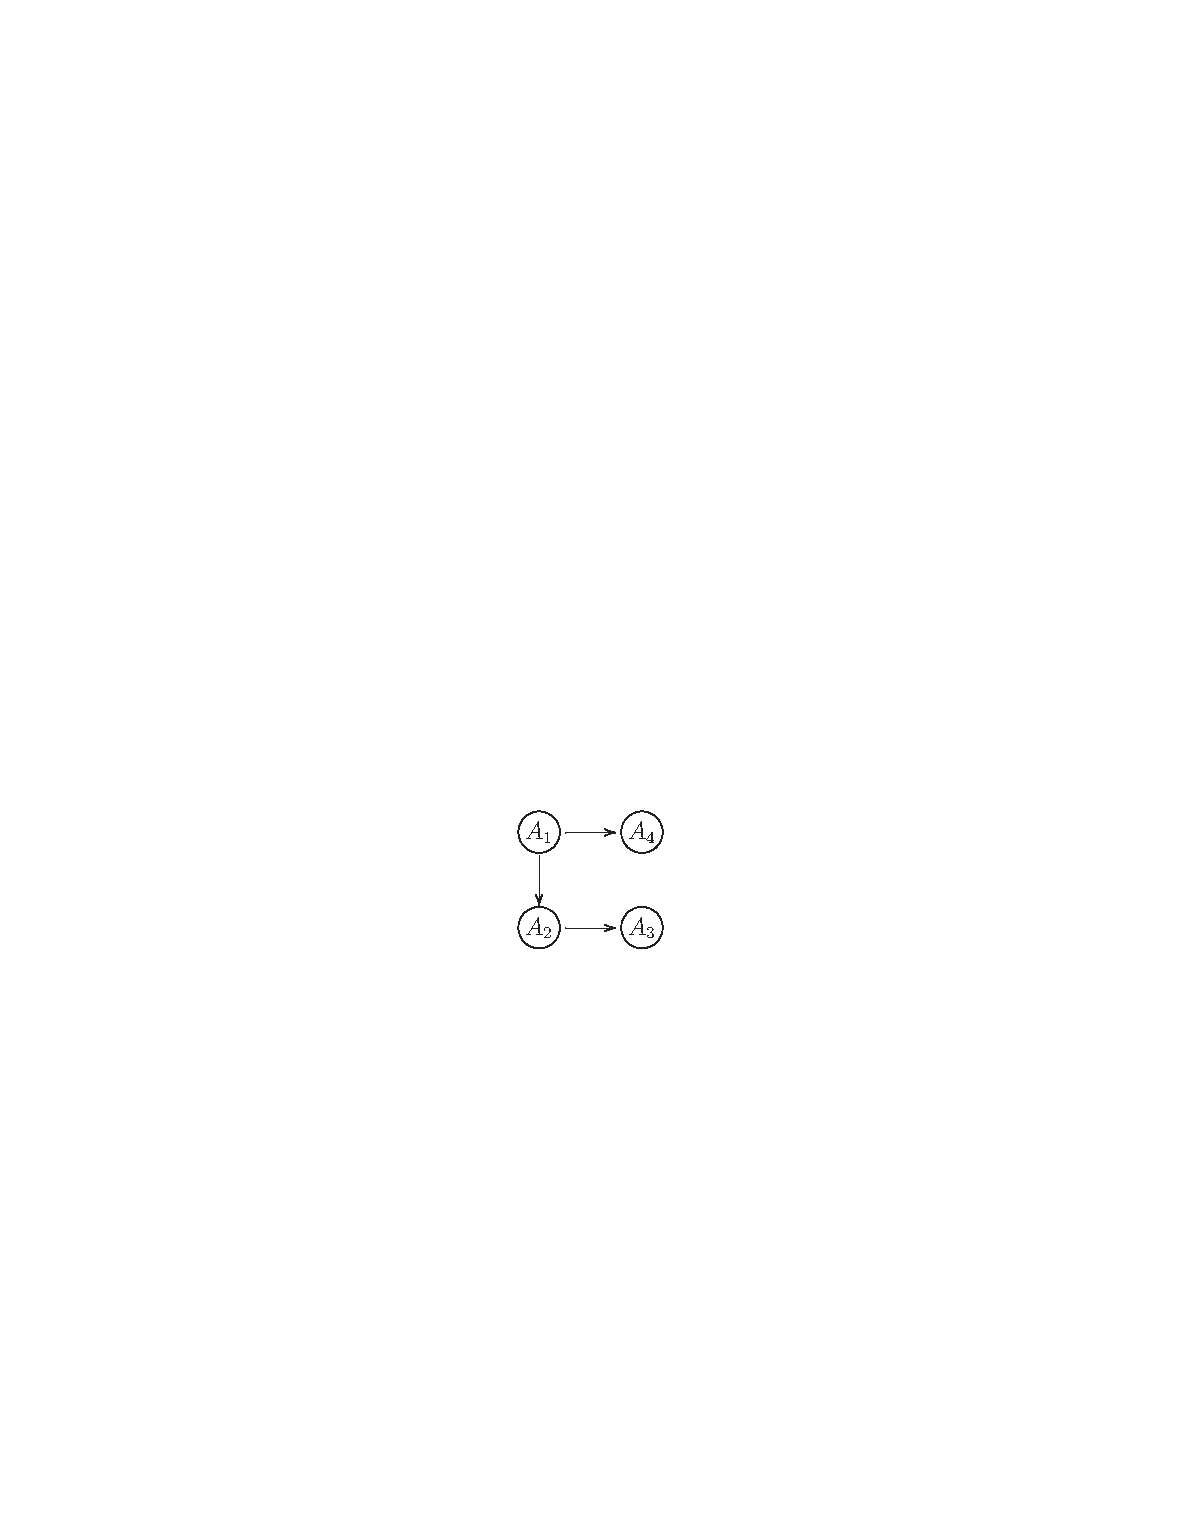
\includegraphics[height=2cm]{images/GraphCase3.pdf}
	\end{center}
	Here the information exchange topology has a 
	{\textcolor{green!40!black}{\fontsize{13}{15}\textbf{leader– follower structure}}}
	and L can be written as an upper diagonal matrix. 
 \end{column}
\end{columns}
We know that zero is a simple eigenvalue of L and all non-zero eigenvalues are real. 
So, we know that {\textcolor{green!40!black}{\fontsize{13}{15}\textbf{consensus is achieved asymptotically}}}.
\vskip 0.3cm
\end{frame}

%%%%%%%%%%%%%%%%%%%%%%
\begin{frame}{Case 4A}

\begin{columns}
 \begin{column}{.70\textwidth}
	\begin{center}
		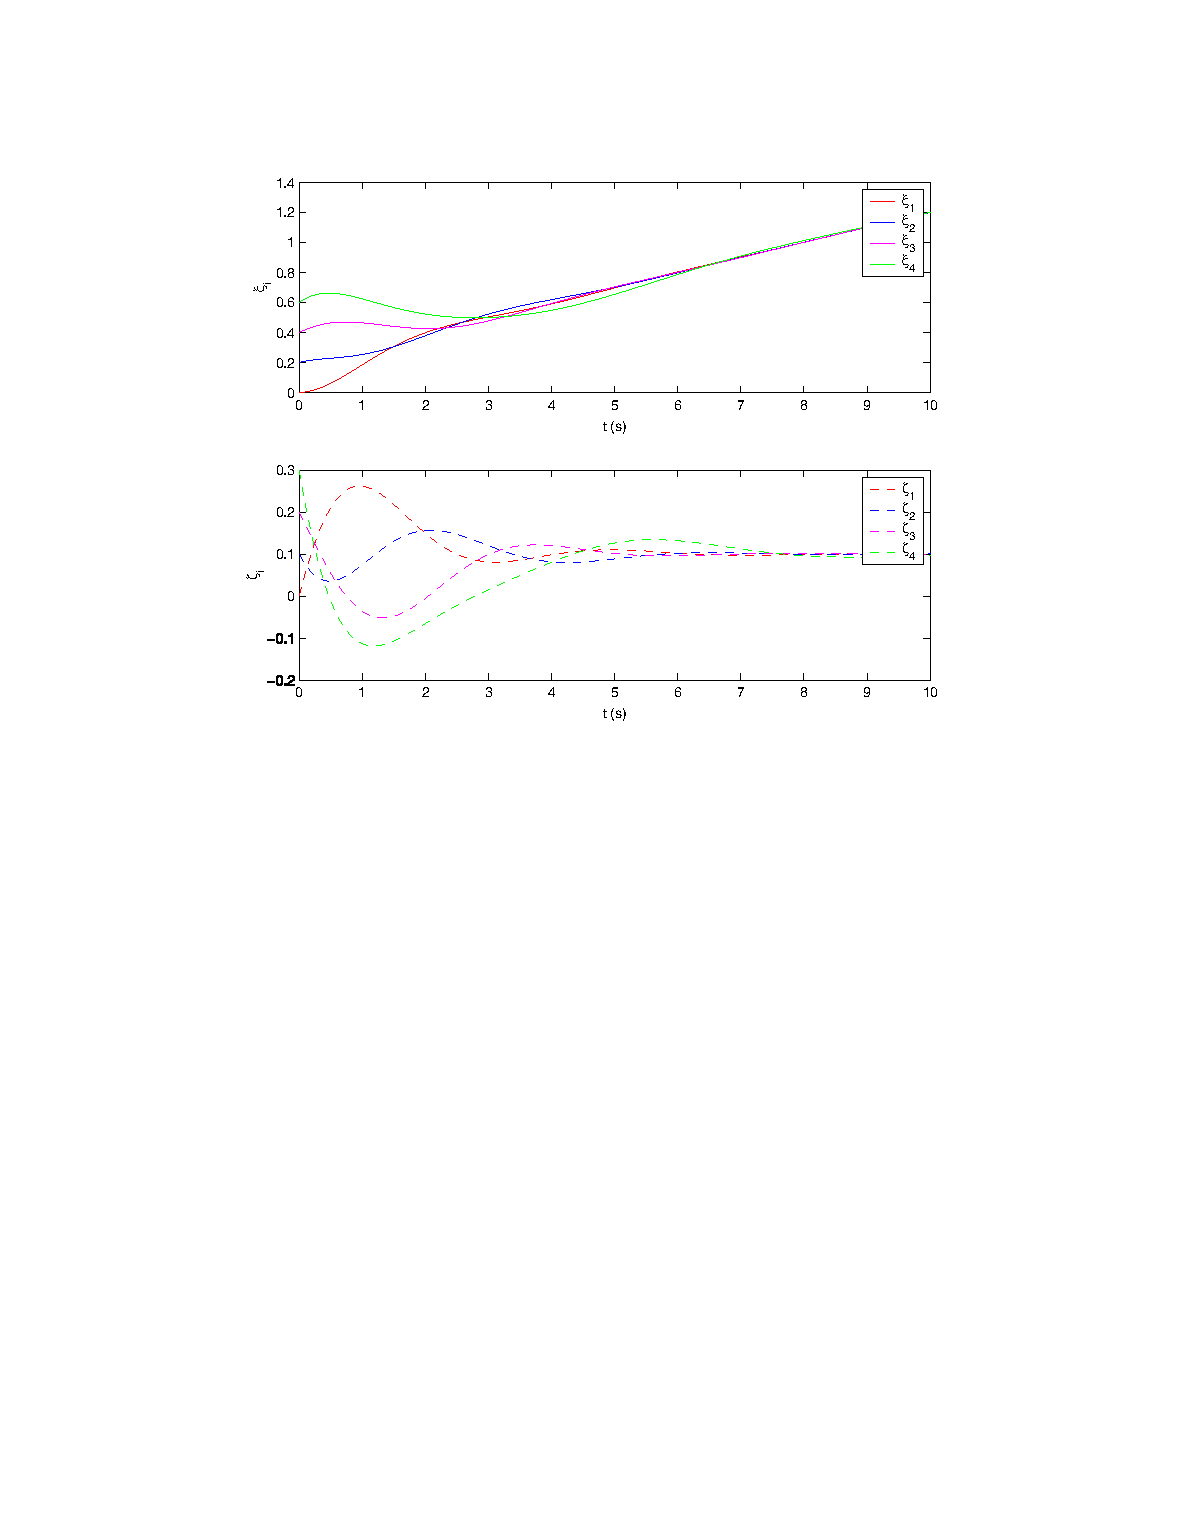
\includegraphics[height=6cm]{images/StatesCase4A.pdf}
	\end{center}
	\vskip 0.3cm
 \end{column}
 \begin{column}{.30\textwidth}
 	\vskip 0.3cm
	\begin{center}
		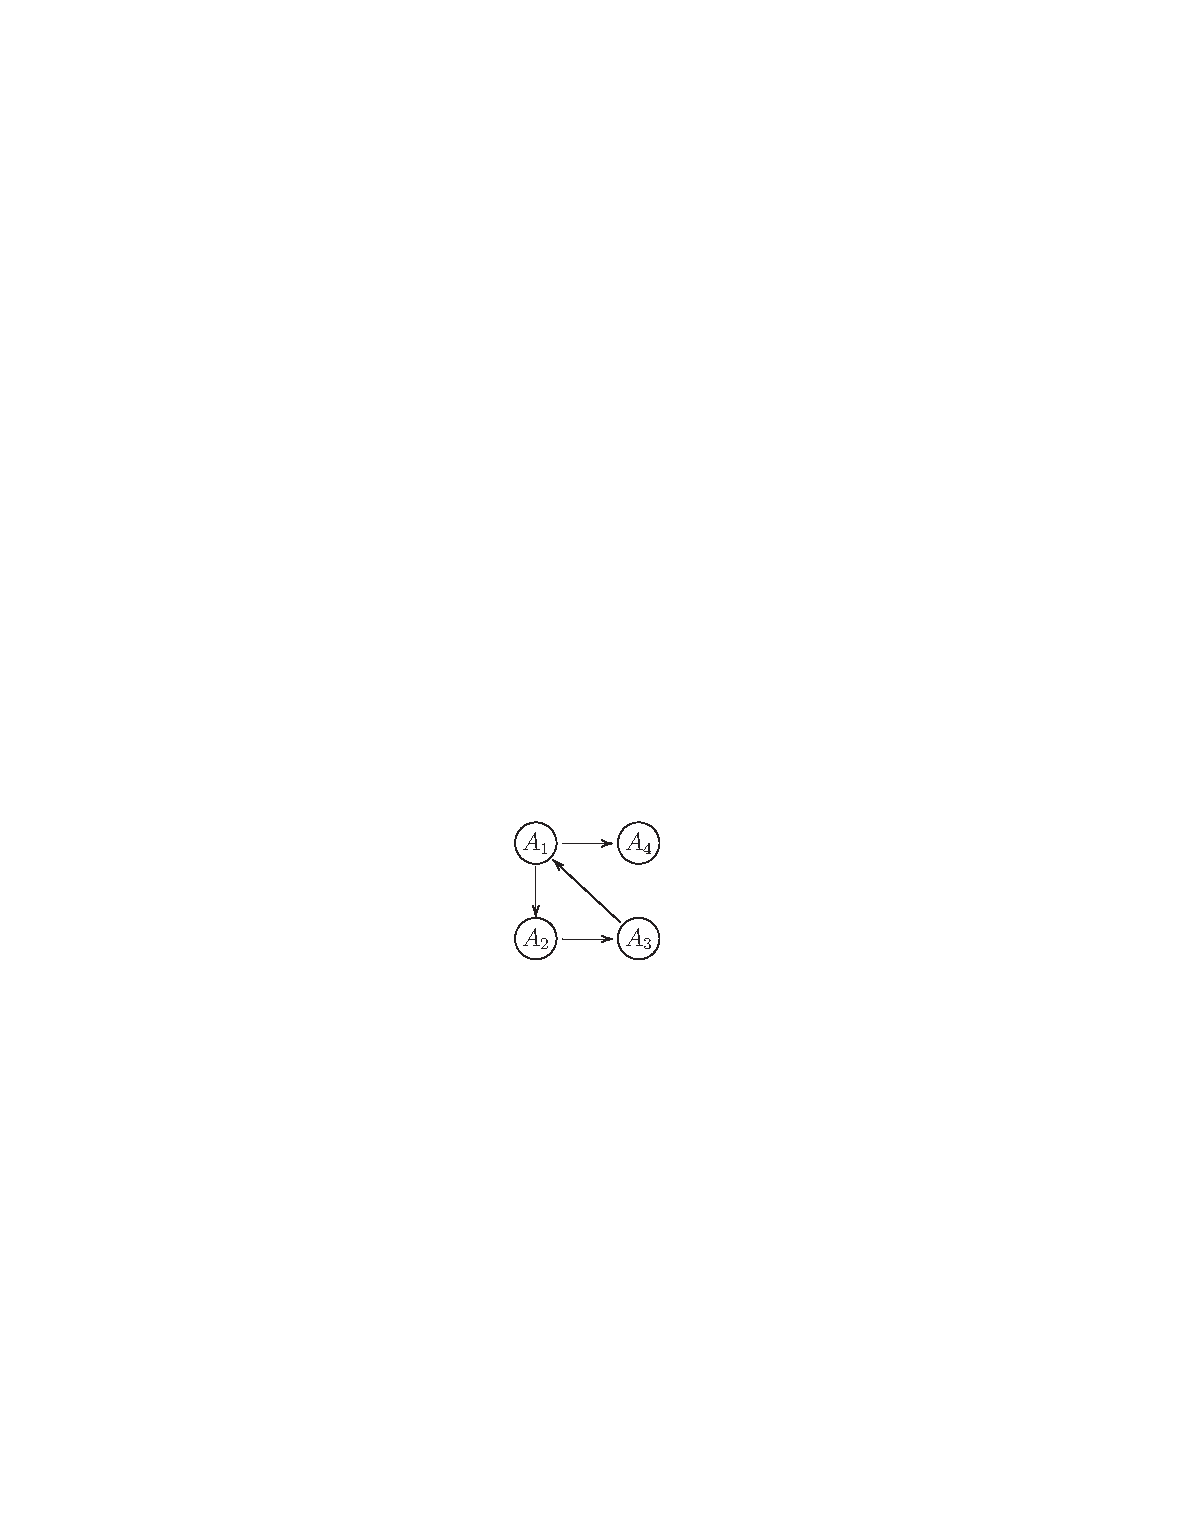
\includegraphics[height=2cm]{images/GraphCase4.pdf}
	\end{center}
	Having a (directed) spanning tree is a necessary condition for  
	{\textcolor{green!40!black}{\fontsize{13}{15}\textbf{consensus}}},
	but  it {\textcolor{green!40!black}{\fontsize{13}{15}\textbf{may not be achieved}}}.
 \end{column}
\end{columns}
In this case  {\textcolor{green!40!black}{\fontsize{13}{15}\textbf{consensus can be reached for $\gamma = 1$}}}, 
 but could not be reached for smaller $\gamma$.
\vskip 0.3cm
\end{frame}

%%%%%%%%%%%%%%%%%%%%%%
\begin{frame}{Case 4B}

\begin{columns}
 \begin{column}{.70\textwidth}
	\begin{center}
		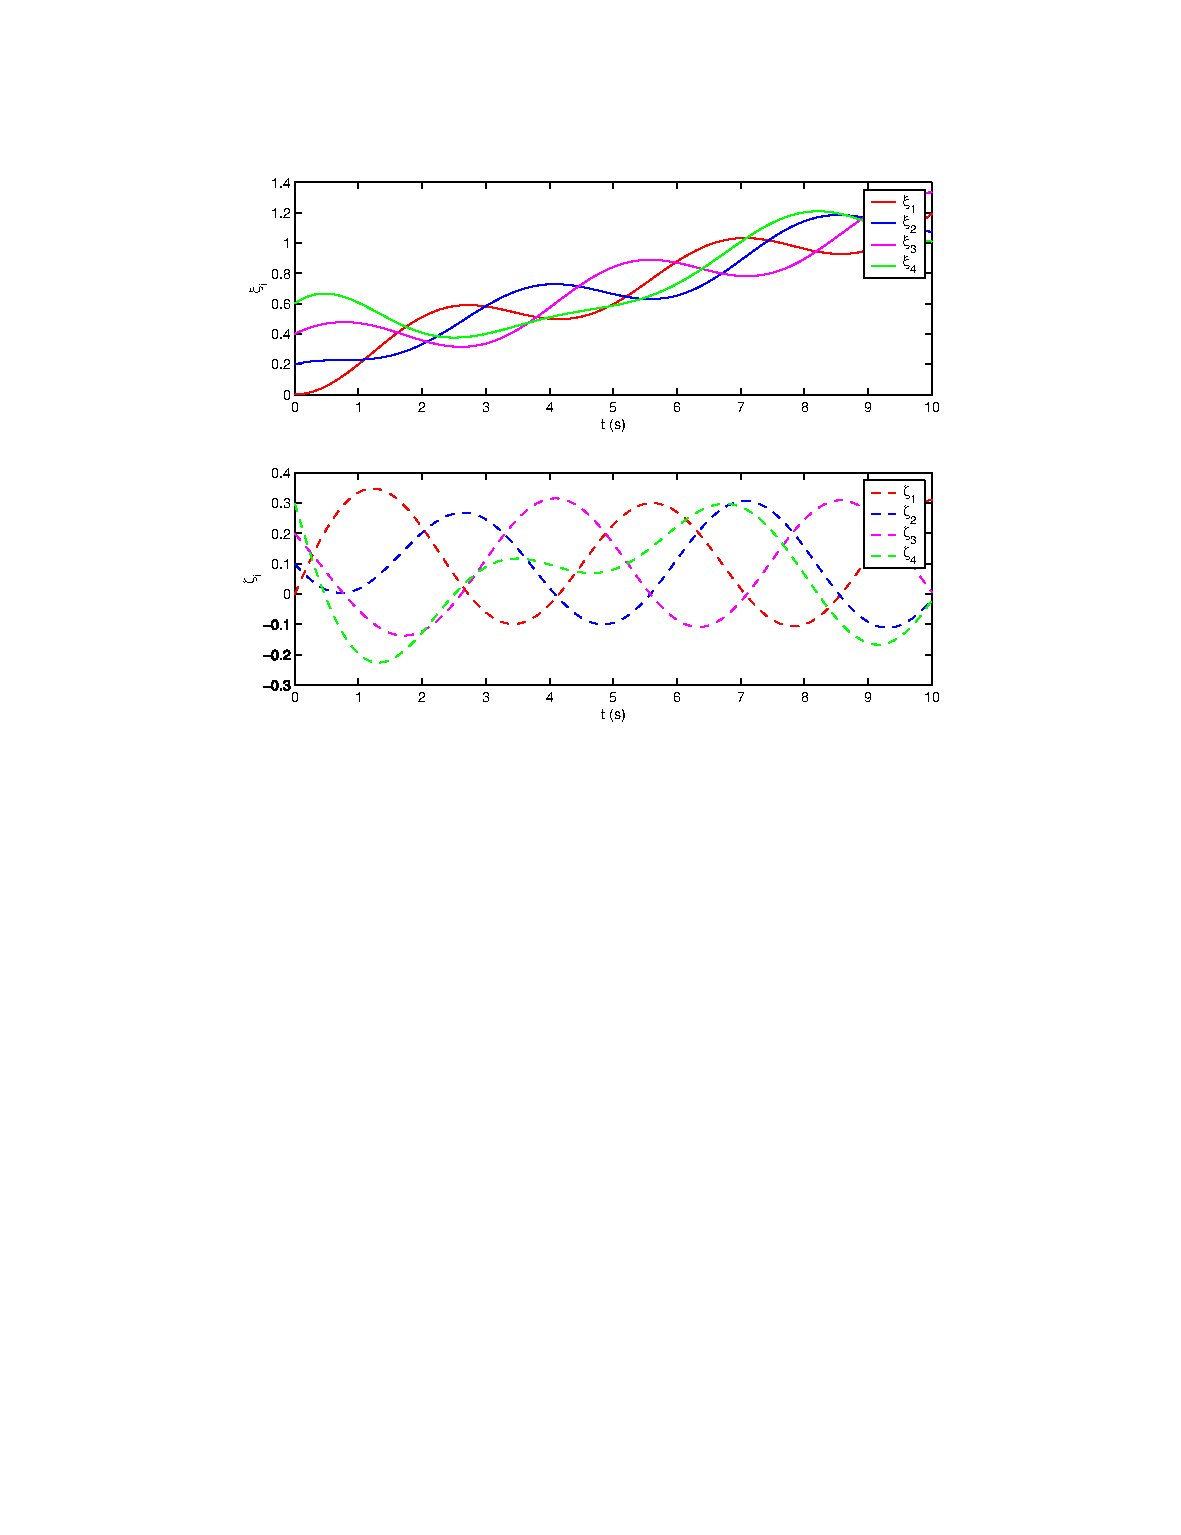
\includegraphics[height=6cm]{images/StatesCase4B.pdf}
	\end{center}
	\vskip 0.3cm
 \end{column}
 \begin{column}{.30\textwidth}
 	\vskip 0.3cm
	\begin{center}
		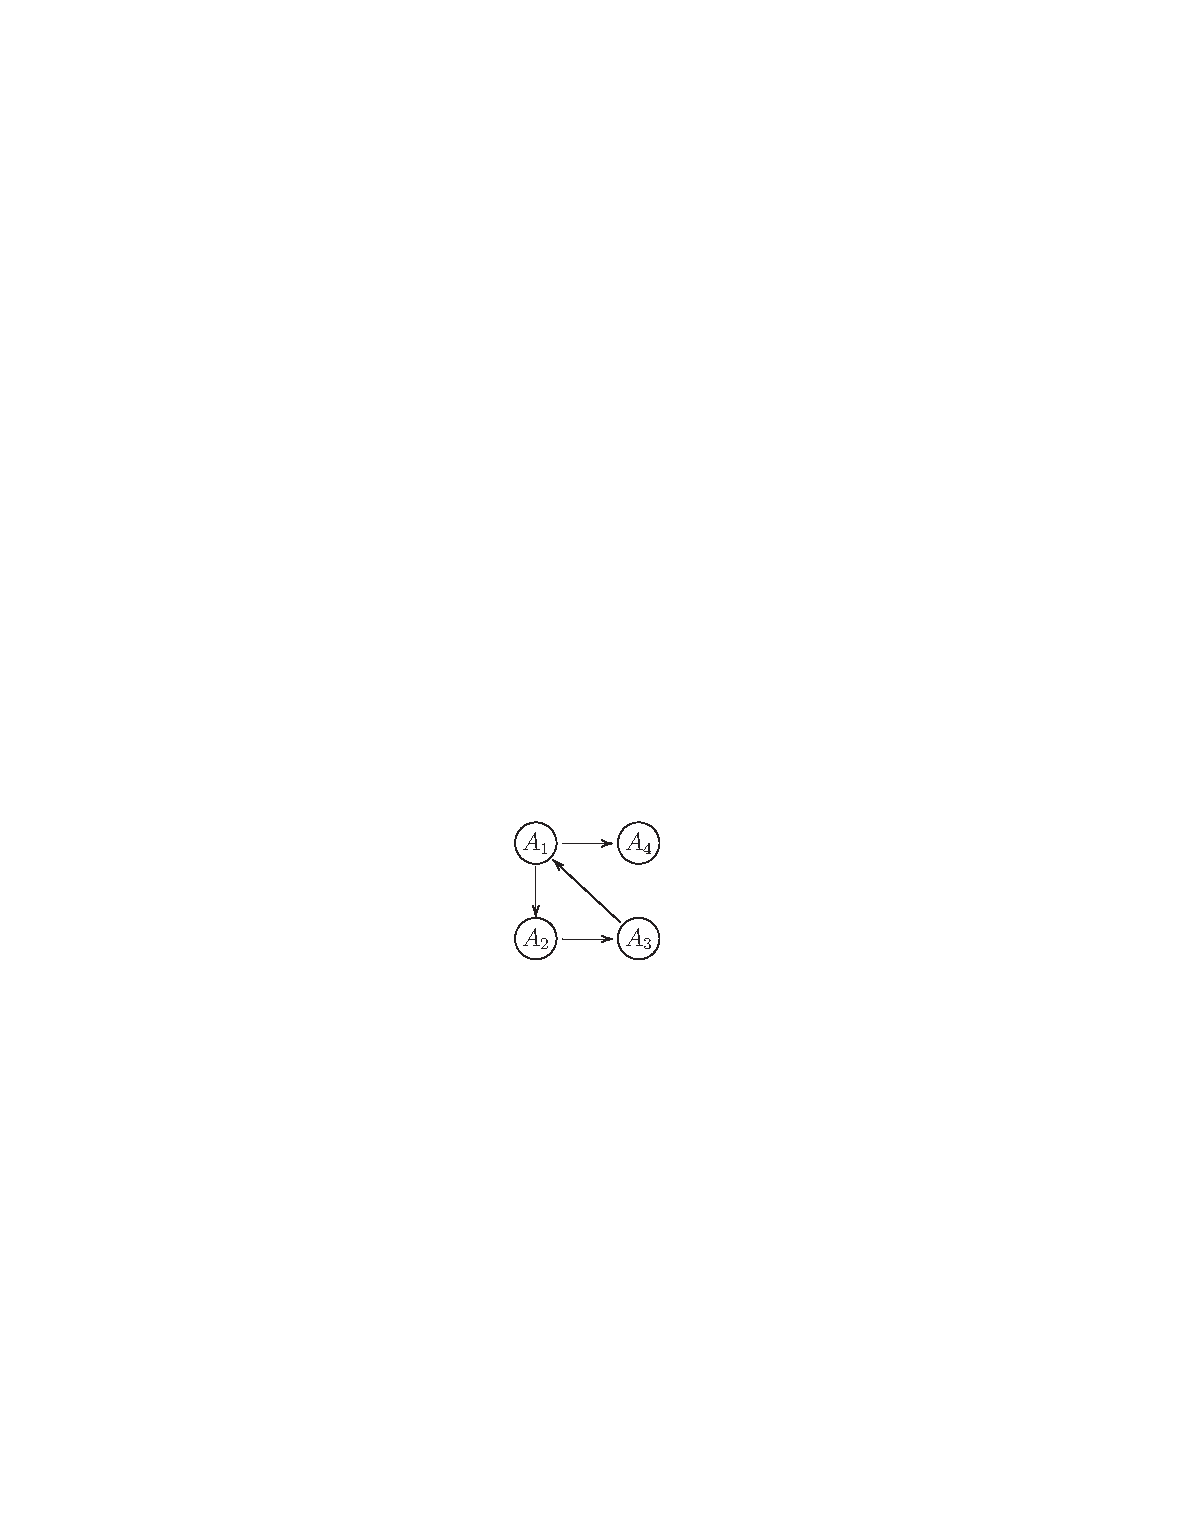
\includegraphics[height=2cm]{images/GraphCase4.pdf}
	\end{center}
	Having a (directed) spanning tree is a necessary condition for  
	{\textcolor{green!40!black}{\fontsize{13}{15}\textbf{consensus}}},
	but  it {\textcolor{green!40!black}{\fontsize{13}{15}\textbf{may not be achieved}}}.
 \end{column}
\end{columns}
In this case  {\textcolor{green!40!black}{\fontsize{13}{15}\textbf{consensus cannot be reached for $\gamma = 0.4$}}}.
\vskip 0.3cm
\end{frame}


%%%%%%%%%%%%%%%%%%%%%%
\begin{frame}{Conclusions}
\vskip 0.5cm
\begin{block}{}
If  $-L$ has a simple zero eigenvalue and all the other eigenvalues are real, 
consensus protocol achieves consensus for any $\gamma > 0$:
\end{block}
\vskip 0.1cm
\begin{block}{}
Matrix $L$ of a directed weighted graph has a simple zero eigenvalue and
all the other eigenvalues have positive real parts if and only if the graph has a (directed) spanning tree.
\end{block}
\vskip 0.1cm
\begin{block}{}
Consensus protocol achieves consensus asymptotically 
if the information exchange topology has a (directed) spanning tree and:
$$
\gamma > \max_{\mu_i \neq 0} {\sqrt{ \frac{ 2 }{\lvert \mu_i \rvert \cos{ \left( \frac{\pi}{2} - \tan^{-1}{ \frac{-Re(\mu_i)}{Im(\mu_i)} } \right) }}}}
$$
\end{block}
\end{frame}